%%%%%%%% ICML 2019 EXAMPLE LATEX SUBMISSION FILE %%%%%%%%%%%%%%%%%

\documentclass{article}

% Recommended, but optional, packages for figures and better typesetting:
\usepackage{microtype}
\usepackage{graphicx}
\usepackage{subfigure}
\usepackage{booktabs} % for professional tables
\usepackage{natbib}
\usepackage{graphicx}
\usepackage{amsmath}
\usepackage{amssymb}
\usepackage{multirow}
%\usepackage{subcaption}

% hyperref makes hyperlinks in the resulting PDF.
% If your build breaks (sometimes temporarily if a hyperlink spans a page)
% please comment out the following usepackage line and replace
% \usepackage{icml2019} with \usepackage[nohyperref]{icml2019} above.
\usepackage{hyperref}

% Attempt to make hyperref and algorithmic work together better:
\newcommand{\theHalgorithm}{\arabic{algorithm}}

% Use the following line for the initial blind version submitted for review:
\usepackage{icml2019}

% If accepted, instead use the following line for the camera-ready submission:
%\usepackage[accepted]{icml2019}

% The \icmltitle you define below is probably too long as a header.
% Therefore, a short form for the running title is supplied here:
\icmltitlerunning{Bin Packing}

\begin{document}

\twocolumn[
\icmltitle{Bin Packing}

% It is OKAY to include author information, even for blind
% submissions: the style file will automatically remove it for you
% unless you've provided the [accepted] option to the icml2019
% package.

% List of affiliations: The first argument should be a (short)
% identifier you will use later to specify author affiliations
% Academic affiliations should list Department, University, City, Region, Country
% Industry affiliations should list Company, City, Region, Country

% You can specify symbols, otherwise they are numbered in order.
% Ideally, you should not use this facility. Affiliations will be numbered
% in order of appearance and this is the preferred way.
\icmlsetsymbol{equal}{*}

\begin{icmlauthorlist}
\icmlauthor{Bharathan Balaji}{equal,to}
\icmlauthor{Jordan Bell-Masterson}{equal,goo}
\icmlauthor{Chun Ye}{equal,ed}
\end{icmlauthorlist}

\icmlaffiliation{to}{AWS Sagemaker RL}
\icmlaffiliation{goo}{SCOT SimEx}
\icmlaffiliation{ed}{GDS MOP}

\icmlcorrespondingauthor{Bharathan Balaji}{bhabalaj@amazon.com}
%\icmlcorrespondingauthor{Eee Pppp}{ep@eden.co.uk}

% You may provide any keywords that you
% find helpful for describing your paper; these are used to populate
% the "keywords" metadata in the PDF but will not be shown in the document
\icmlkeywords{Machine Learning, ICML}

\vskip 0.3in
]

% this must go after the closing bracket ] following \twocolumn[ ...

% This command actually creates the footnote in the first column
% listing the affiliations and the copyright notice.
% The command takes one argument, which is text to display at the start of the footnote.
% The \icmlEqualContribution command is standard text for equal contribution.
% Remove it (just {}) if you do not need this facility.

%\printAffiliationsAndNotice{}  % leave blank if no need to mention equal contribution
\printAffiliationsAndNotice{\icmlEqualContribution} % otherwise use the standard text.

\begin{abstract}
\end{abstract}

\section{Bin Packing}
\label{binpacking}

In the classic bin packing problem, we fit given items of varying sizes into as few fixed size bins as possible. In the online stochastic version of this problem, each item arrives one at a time and its size varies according to an unknown distribution. 
%We formulate the problem as a Markov Decision Process and compare a reinforcement learning algorithms against a well-known baseline (Sum of Squares) that asymptotically converges to a good solution regardless of the item size distribution. 

Our motivation for exploring the bin packing problem is in the many applications to operations research and computer science problems at Amazon. 
%For instance, in the cutting stock problem, a manufacturer produces cables of fixed lengths, customer orders that with specific cable lengths arrive and must be served online from the available inventory.  The goal is to serve the demand while minimizing the rate of production of cables. In appointment scheduling, requests for appointments arrive online and must be scheduled in a future day with available slots. Here appointments correspond to items, and the office hours during a working day correspond to bins. 
In Amazon's fulfillment and transportation operations, for example, bin packing is related to the order assignment problem, to tote packing, to trailer truck packing, among others.  
%In this problem, customers orders arrive online and must be assigned to a ship method that connects an Amazon FC to the customer's location. For candidate each assignment, the order items would utilize our transportation resources (truck/plane space, labor). The task is to fulfill all orders while utilizing the least number of transportation resources.
In AWS, bin packing is related to placement of virtual machines on servers and allocating memory to processes within a machine. 
\ifx 3d bin packing has many applications within Amazon operations from packing of picked items into totes to the packing of packages onto trailers. The need to use as few bins as possible directly translates into cost savings. \emph{Bharath} can you write about the VM
\fi

\subsection{Problem Formulation} \label{sec: bin_packing_prob_form}
In a stochastic bin packing problem, items arrive in an online fashion in each time period $t = 1, \ldots, T$. Items can be of different types $j \in \{1,...,J\}$. The size of type $j$ is $s_j$ and the probability that an item is of type $j$ is $p_j$. Without loss of generality, we assume item types are indexed in the increasing order of their size: $s_1 < s_2 < ... < s_J$. Upon arrival, the item needs to be packed into a bin of size $B$ (we assume that $s_J < B < \infty$). A packing is considered feasible if the total size of the items packed in each bin does not exceed the bin size. The task is to minimize the number of bins used to pack all of the items within the time horizon. We assume the item sizes $s_j$ and bin size $B$ are integers. We assume the number of bins one can open is unlimited and denote the sum of item sizes in a bin as \emph{level} $h$. After $t$ items have been packed, we denote the number of bins at level $h$ as $N_h(t)$, where $h = 1,...,B$. 

It can be shown that minimizing the number of non-empty bins is equivalent to minimizing the total waste (i.e. empty space) in the partially filled bins. Hence our objective is to minimize waste at any point in time:

\begin{equation}
\label{waste}
W(t) \triangleq \sum_{h=1}^{B-1} N_h(t)(B-h) 
\end{equation}

\noindent We use $W^{A}_{F}(t)$ to denote the total waste after step $t$ of algorithm $A$ when the input samples come from distribution $F$. To train our RL algorithm, we define the cumulative reward function to be $W^{RL}_{F}(t)$. Courcoubetis and Weber \cite{courcobetis1990stability} showed that any discrete distribution falls into one of three categories based on expected distribution $E[W^{OPT}_{F}(t)]$.
\begin{enumerate}
	\item Linear waste (LW): $E[W^{OPT}_{F}(t)] = \Theta(t)$, e.g. $B = 9$, two item types of size $\{2,3\}$ with probability $\{0.8, 0.2\}$ respectively.
	\item Perfectly Packable (PP):  $E[W^{OPT}_{F}(t)] = \Theta(\sqrt{t})$, e.g.  $B = 9$, two item types of size $\{2,3\}$ with probability $\{0.75, 0.25\}$ respectively.
	\item PP with bounded waste (BW): $E[W^{OPT}_{F}(t)] = \Theta(1)$, e.g. $B = 9$, two item types of size $\{2,3\}$ with probability $\{0.5, 0.5\}$ respectively.
\end{enumerate}
We will train an RL policy for the above example from each of the three distribution types and compare our policy to the baseline.


\subsection{Related Work}
Bin packing is a very well studied problem in the operations research and computer science literature. 
%Some applications include: loading trucks subject to weight/volume restrictions, to packing television commercials into station breaks, to stock-cutting problems, where items of varying lengths must be cut from some raw materials, e.g. cable, lumber, or paper of a standard size. 
The problem is already NP-hard in its basic form. As a result, many of the classical approaches to bin packing analyze the performance of approximation algorithms. We refer the readers to the survey of Coffman et. al \cite{Coffmanetal2013} for algorithmic approaches to classical bin packing and its generalizations.   

For online bin packing, simple heuristics such as Best Fit is known to use at most $1.7$ times the optimal number of bins in the worst case \cite{Johnsonetal1974}. 
%This paper focuses on the asymptotic performance of online stochastic bin packing. Many research papers in this vein analyze the performance of common (distributional agnostic) heuristics such as First Fit and Best Fit, and on specific distributions such as uniform \cite{Shor:1986}\cite{Leighton:1986}\cite{coffmanetal1991}\cite{Kenyon1998}\cite{Albers1998} and skewed uniform \cite{KenyonMitzen2000}. A few papers also identify an optimal policy for specific item size distributions, e.g. \cite{Shor1991}. 
The Sum of Squares (SS) heuristic \cite{csirik2006sum} is arguably the state-of-the-art asymptotic bin packing policy when item sizes $\{s_j\}$ and bin size $B$ are integral. It is distributional agnostic and nearly universally optimal (up to constant factors) for types of distributions $F$. %In \cite{csirik2006sum}, it is shown that SS has $O(\sqrt{t})$ waste for PP distribution, matching the optimal. For BW distributions, the waste of SS is $O(\log t)$, which can be reduced to $O(1)$ by learning the support of the distribution. For LW, SS is suboptimal by an additive constant factor i.e. $\Theta(t)$. The sub-optimality can be reduced by learning the item size distribution and solving a LP to fine-tune the heuristic. \cite{gupta2012online} proposed heuristics to obtain $\Theta(\sqrt{t})$ additive sub-optimality for all distributions, inspired by approximate interior-point algorithms for convex optimization.

The simple heuristics described above are distribution agnostic. More sophisticated algorithms learn an empirical estimate of the item size distribution, leverage such distribution to solve a linear program, and use its dual to guide the online policy \cite{AdelmanNem1999}\cite{RheeTalagrand1993}\cite{IyengarSigman2004}. This approach has been extended to solve online packing and covering problems (see e.g. \cite{GuptaMolinaro2014}\cite{AgrawalDevanur2015}).

%Online stochastic bin packing~\cite{gupta2012online}

\subsection{Baseline Algorithm}
We use the well-known Sum of Squares (SS) heuristic~\cite{csirik2006sum} as our baseline algorithm. For the integral item sizes and bin size problem, SS heuristic is nearly universally optimal for all item size distributions and almost distribution-agnostic. When the $t$th item of size $s$ arrives, SS picks a bin of level $h^*$ that minimizes the value of the following sum-of-squares potential:

\begin{equation}
\sum_{h=1}^{B-1} (N_{h}(t))^2. \label{SOS eq}
\end{equation}

\noindent It can be shown that minimizing (\ref{SOS eq}) is equivalent to minimizing:
\begin{equation}
h^* = \underset{h:N_n(t-1)>0}{\arg\min} [N_{h+s}(t-1) - N_h(t-1)], \label{SOS eq1}
\end{equation}

\noindent where, $N_0 = N_B = 0$. Intuitively, SS tries to equalize the number of bins at each level. Due its simplicity, we implemented (\ref{SOS eq1}) version of SS.

\subsection{Reinforcement Learning Algorithm}
We formulate this as a Markov Decision Process, where the state $S_t \in \mathcal{S}$ is current item type $j_t$ and the number of bins at each level: $N_h(n)$, where $h = 1,...,B$. The action $A$ is to pick a bin level which can fit the item.  Thus, the number of actions possible is $B$ with one action for each level and action 0 corresponds to opening a new bag. Initially, all the bins are empty. The reward $R_t$ is the negative of incremental waste as each item is put into bins. If the item is put into an existing bin, the incremental waste will reduce by item size. If the item is put into a new bag, the waste increases by the empty space left in the bag. The agent can take an invalid action by picking a level for which bins do not exist yet. In that case, we give a high negative penalty (-100 in our experiments) and terminate the episode. 

We use the Proximal Policy Optimization (PPO) algorithm~\cite{schulman2017proximal}. PPO is a type of an actor-critic algorithm~\cite{konda2000actor}, where the actor is represented a policy network and takes the environment state as input and the action as the output. The critic is represented by a value network and takes the environment state as input and predicts the cumulative discounted reward that will be obtained from this state. Intuitively, the actor tells the agent how to act and the critic informs the agent how good the action was. 	Initially, the two neural networks are initialized with random weights, i.e. they take random actions, and the agent interacts with the environment to generate a dataset of tuples: $(S_t, A_t, R_t, S_{t+1})$. The dataset is used to update the weights of the two neural networks. The updated neural networks are used to interact with the environment to generate more data and the cycle continues until training stops (22 hours time limit in our experiments). We refer the reader to the original paper for a formal explanation of the algorithm~\cite{schulman2017proximal}.

In our experiments, we use a two-layer neural network with 256 hidden nodes each. The input to both policy and value network is the state, the output of the policy network is a probability of taking an action and the output of value network is a number for predicted value. During training, the agent explores the state space by sampling from the probability distribution of the actions generated by the policy network. During evaluation, the agent takes the action with the highest action probability. We show the hyperparameters we used in Table \ref{table:bin_packing_hyperparam}.

\begin{table}[h!]
	\centering
	\begin{tabular}{ |c|c|c|c| } 
		\hline
		Discount factor & 0.995 & KL coefficient & 1.0 \\ 
		\hline
		Experience Buffer & 320000 & Learning rate & 0.0001 \\
		\hline	
		SGD Mini-batch & 32768 & Epochs & 10 \\
		\hline
		Entropy coefficient & 0 & \# Workers & 7 \\
		\hline
		Episode length & 1000 & clip param & 0.3 \\
		\hline
	\end{tabular}
	\caption{Hyperparameters used in PPO algorithm for Bin Packing}
	\label{table:bin_packing_hyperparam}
\end{table}


\subsection{Results}
For each sample item size distribution (BW, PP, LW) considered in section \ref{sec: bin_packing_prob_form}, we train the RL algorithm (PPO) and compare to the baseline algorithm (SS).  At a high level, by the end of training RL outperforms the baseline irrespective of distribution, and converges to a sensible learned policy structure.
\begin{figure}[h!]
	\centering
	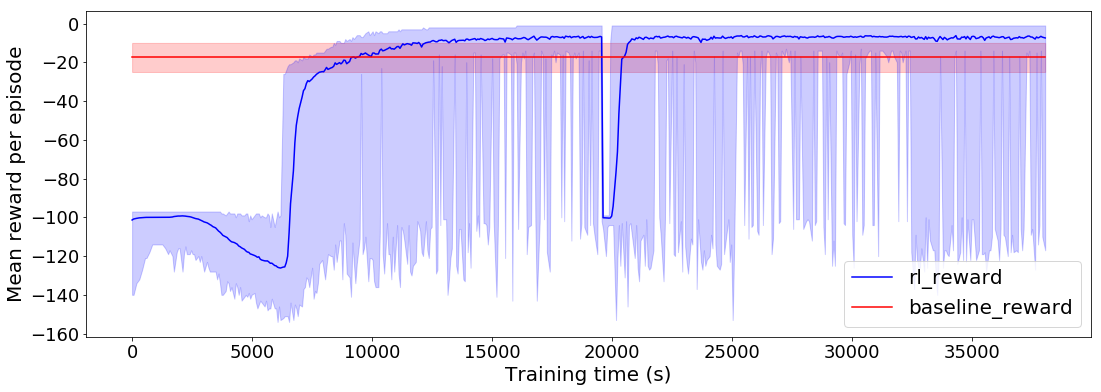
\includegraphics[width=1\linewidth]{images/bin_packing_rl_vs_baseline_bounded_waste_binsize_9.png}
	\caption{RL vs baseline for BW distribution}
	\label{fig:bin_packing_BW_dist}
\end{figure}

\begin{figure}[h!]
	\centering
	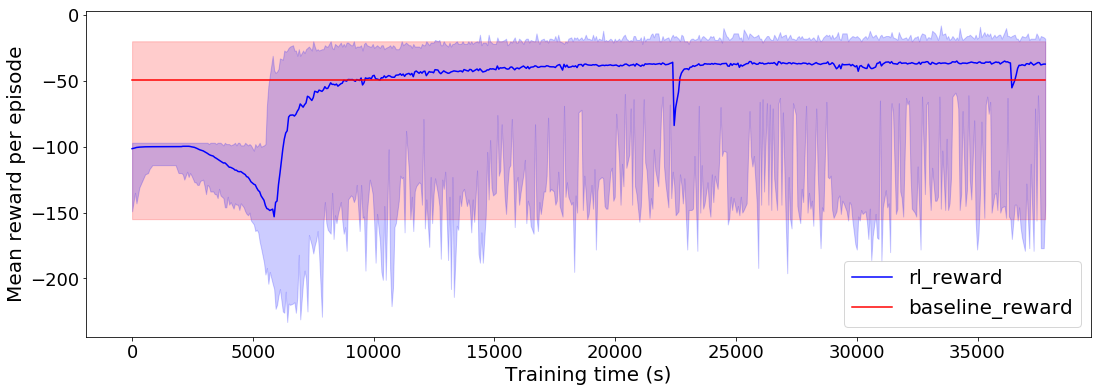
\includegraphics[width=1\linewidth]{images/bin_packing_rl_vs_baseline_perfect_pack_binsize_9.png}
	\caption{RL vs baseline for PP distribution}
	\label{fig:bin_packing_PP_dist}
\end{figure}

\begin{figure}[h!]
	\centering
	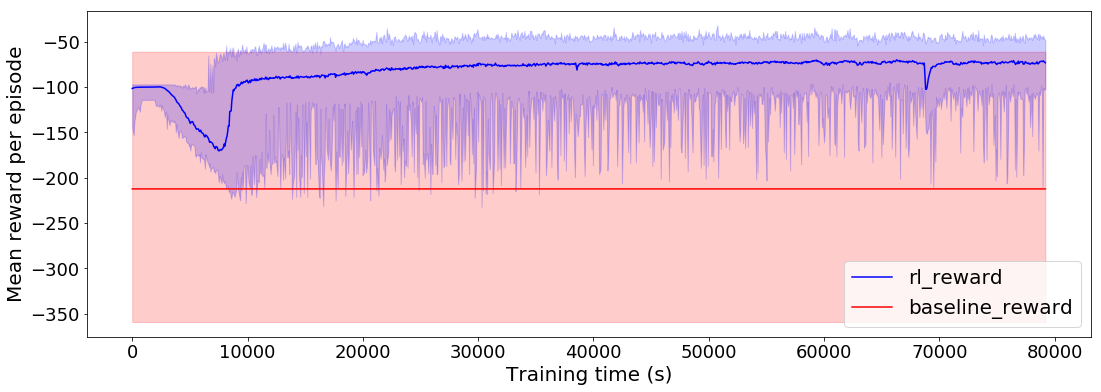
\includegraphics[width=1\linewidth]{images/bin_packing_rl_vs_linear_waste_binsize_9.png}
	\caption{RL vs baseline for LW distribution}
	\label{fig:bin_packing_LW_dist}
\end{figure}
Figures \ref{fig:bin_packing_LW_dist} through \ref{fig:bin_packing_BW_dist} plot the reward function of the RL policy in training (blue) vs the baseline (red) for different item size distributions (BW, PP, and LW) as a function of training time (measured in seconds). In particular, the solid lines represent the mean reward of each policy, and the shaded bands represent the min/max rewards of each policy.  By the end of training, RL outperforms the baseline policy for all three item size distributions. In particular, the reward gap between RL and baseline is the largest for LW distribution (which is expected, as SS is known to be suboptimal for LW distribution). The min reward of RL sometimes falls below that of SS as RL tries to explore different actions in training.

In Table \ref{table:bin_packing_RL_baseline_comp}, we inspect numerically the trained RL policy vs. baseline.  Note that the exploration parameters are turned off for the trained RL policy.  Supporting what we observed in the initial figures, this table shows the final RL policy outperforming the baseline for each distribution.
\begin{table}[h!]
	\centering
	\begin{tabular}{ |c|c|c|c| } 
		\hline
		Algorithm & Item Size Dist. & Mean & Std. Dev. \\ 
		\hline
		\multirow{3}{4em}{RL}  & Bounded Waste & -5.75  & 3.21 \\ 
		& Perfectly Packable & -36.5 & 14.2 \\
		& Linear Waste  &  -73.08 &  8.56 \\
		\hline	
		\multirow{3}{4em}{SS} & Bounded Waste & -17.27  & 3.21 \\ 
		& Perfectly Packable & -50.18 & 28.59 \\ 
		& Linear Waste &  -212.24 & 68.66 \\ 
		\hline
	\end{tabular}
	\caption{Comparison between RL and baseline.}
	\label{table:bin_packing_RL_baseline_comp}
\end{table}

Finally, we inspect the relative structure of the policies to ensure that RL is learning a sensible solution.  In particular, we plot the state variable values as a function of the number of steps in an episode. Intuitively, the integral of these plots represents the waste, which we want to minimize.  An optimal policy should show a (relatively) flat surface.

In the LW distribution case, we see that the baseline policy leaves more open bins at a lower fullness, whereas RL only leaves open bins at level 8 (which cannot be closed once they reach that level).

In the PP distribution case, we see that RL converges to a structure very similar to the baseline, but again with a little more smoothness prior to bin-level 8.
Finally, in the BW distribution case, RL is most impressive relative to the baseline, as RL avoids entirely the bin-level 8 trap and achieves a nearly perfectly flat surface.  Together, these plots show that RL is learning a policy structure similar to what we expect from the baseline, but with some improvements toward optimality (especially in the BW case).

\begin{figure}[h!]
	\centering
	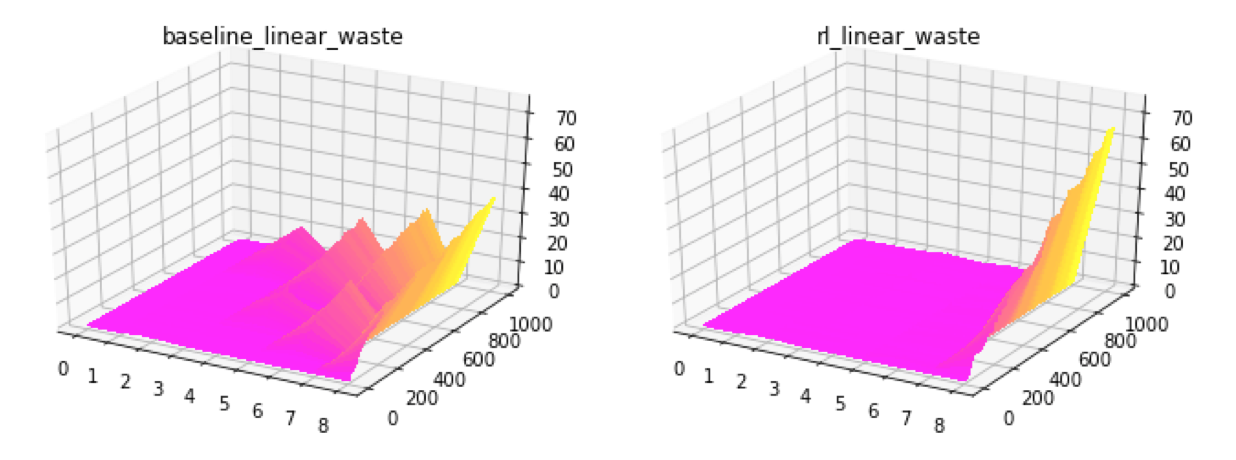
\includegraphics[width=1\linewidth]{images/linear_waste_sol.png}
	\caption{RL vs baseline solution for LW distribution}
	\label{fig:bin_packing_LW_dist}
\end{figure}

\begin{figure}[h!]
	\centering
	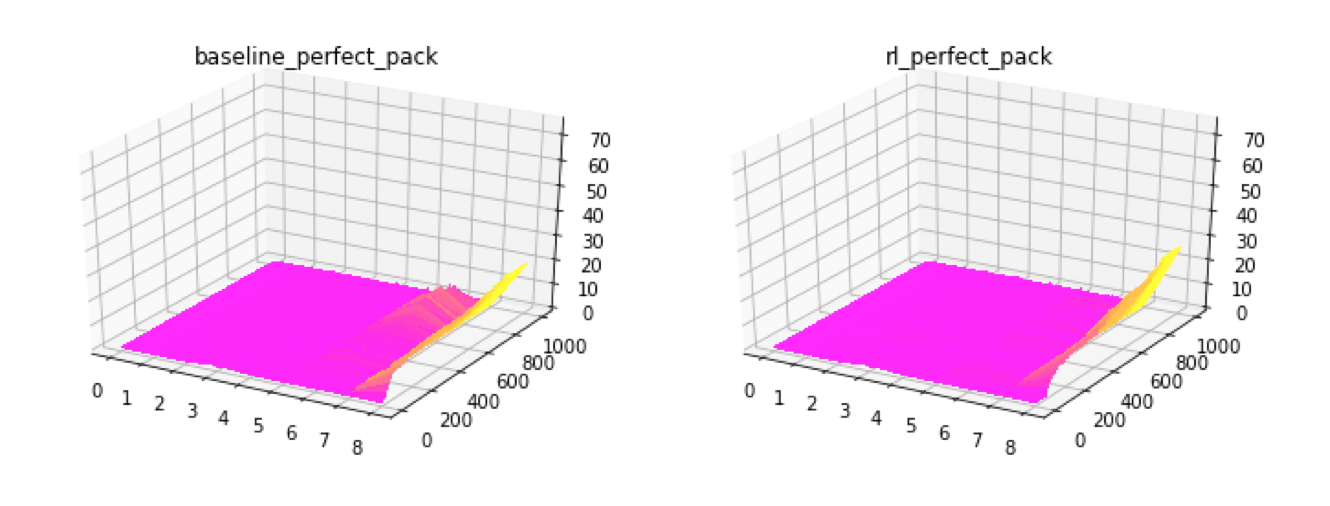
\includegraphics[width=1\linewidth]{images/perfect_packing_sol.png}
	\caption{RL vs baseline solution for PP distribution}
	\label{fig:bin_packing_BW_dist}
\end{figure}

\begin{figure}[h!]
	\centering
	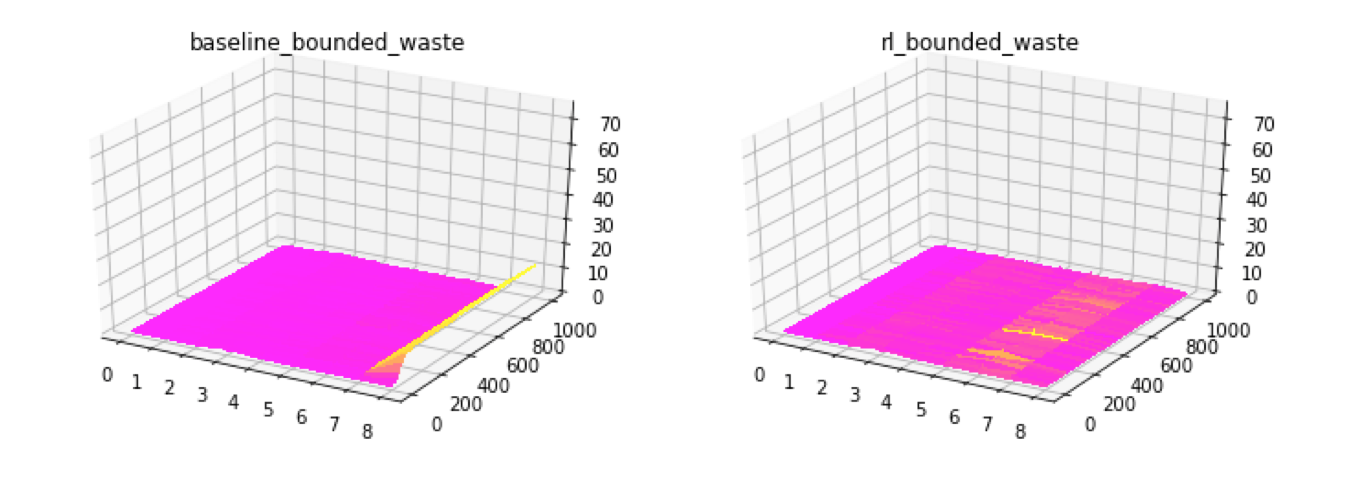
\includegraphics[width=1\linewidth]{images/bounded_waste_sol.png}
	\caption{RL vs baseline solution for BW distribution}
	\label{fig:bin_packing_BW_dist}
\end{figure}

%Note that for all items size distributions, solution returned by RL uses many more bins at fullness level of 8 or 9 (recall that bin size is 9), whereas SS also uses more bins at lower fullness level compared to RL. 
Below is an example of the frequency of bins of different fullness level for one run of RL vs baseline for each of the three size distributions:

\begin{table}[h!]
	\centering
	\begin{tabular}{ |c|cc|cc|cc| } 
		\hline
		Fullness Level&LW&&PP&&BW& \\
		\hline
		& RL&SS&RL&SS&RL&SS \\
		\hline
		
		2 & 0 & 1 & 0 & 0 & 0 & 0 \\
		\hline
		3 & 0 & 0 & 2 & 0 & 0 & 0 \\
		\hline
		4 & 0 & 9 & 0 & 1 & 0 & 0 \\
		\hline
		5 & 1 & 0 & 0 & 0 & 0 & 0 \\
		\hline
		6 & 0 & 16 & 0 & 9 & 0 & 2 \\
		\hline
		7 & 0 & 0 & 0 & 0 & 1 & 0 \\
		\hline
		8 & 78 & 27 & 19 & 18 & 0 & 10 \\
		\hline
		9 & 173 & 208 & 233 & 229 & 278 & 271 \\
		\hline
		Total Reward & -82 & -127 & -31 & -50 & -2 & -16 \\
		\hline
	\end{tabular}
	\caption{Comparison between RL and baseline solutions.}
	\label{table:bin_packing_RL_baseline_sol_comp}
\end{table}
\ifx
\begin{table}[h!]
	\centering
	\begin{tabular}{ |c|c|c| } 
		\hline
		Packing Type & RL & SS \\ 
		\hline
		2 & 0 & 1  \\ 
		\hline
		2,2 & 0 & 9 \\
		\hline
		2,3 & 1 & 0 \\
		\hline
		2,2,2 & 0 & 16 \\   
		\hline
		2,2,2,2 & 76 & 26 \\
		\hline
		2,3,3 & 2 & 1 \\
		\hline
		2,2,2,3 & 169 & 206 \\
		\hline
		3,3,3 & 4 & 2 \\
		\hline
		Total Reward & -82 &-127 \\
		\hline
	\end{tabular}
\end{table}

\begin{table}[h!]
	\centering
	\begin{tabular}{ |c|c|c| } 
		\hline
		Packing Type & RL & SS \\ 
		\hline
		3 & 2 & 0 \\
		\hline
		2,2 & 0 & 1 \\
		\hline
		2,2,2 & 0 & 9 \\   
		\hline
		3,3 & 0 & 0 \\
		\hline
		2,3,3 & 3 & 3 \\
		\hline
		2,2,2,2 & 16 & 15 \\
		\hline
		2,2,2,3 & 226  & 215 \\
		\hline
		3,3,3 & 7 & 14 \\
		\hline
		Total Reward & -31 &-50 \\
		\hline
	\end{tabular}
\end{table}

\begin{table}[h!]
	\centering
	\begin{tabular}{ |c|c|c| } 
		\hline
		Packing Type & RL & SS \\ 
		\hline
		2,2,2 & 0 & 1 \\   
		\hline
		3,3 & 0 & 1 \\
		\hline
		2,2,3 & 1 & 0 \\
		\hline
		2,3,3 & 0 & 10 \\
		\hline
		2,2,2,3 & 163 & 152 \\
		\hline
		3,3,3 & 115 & 119 \\
		\hline
		Total Reward & -2 &-16 \\
		\hline
	\end{tabular}
\end{table}
\fi



% In the unusual situation where you want a paper to appear in the
% references without citing it in the main text, use \nocite
\nocite{langley00}

\bibliography{refs_bin_packing}
\bibliographystyle{icml2019}


\end{document}


% This document was modified from the file originally made available by
% Pat Langley and Andrea Danyluk for ICML-2K. This version was created
% by Iain Murray in 2018, and modified by Alexandre Bouchard in
% 2019. Previous contributors include Dan Roy, Lise Getoor and Tobias
% Scheffer, which was slightly modified from the 2010 version by
% Thorsten Joachims & Johannes Fuernkranz, slightly modified from the
% 2009 version by Kiri Wagstaff and Sam Roweis's 2008 version, which is
% slightly modified from Prasad Tadepalli's 2007 version which is a
% lightly changed version of the previous year's version by Andrew
% Moore, which was in turn edited from those of Kristian Kersting and
% Codrina Lauth. Alex Smola contributed to the algorithmic style files.
